% !TeX root = proyecto.tex

%=========================================================
\chapter{Modelo del alcance}
\label{cap:alcance}

\cdtInstrucciones{
	Indique un resumen que describa el contenido del capítulo.
}
	
%---------------------------------------------------------
\section{Análisis de la problemática}

\cdtInstrucciones{
	Indique en un párrafo o dos el contenido y organización de la problemática.
}
% - - - - - - - - - - - - - - - - - - - - - - - - - - - - 
\subsection{Contexto del proyecto}

\cdtInstrucciones{
	Indique los antecedentes, contexto y características relevantes necesarios para comprender la problemática a resolver.
}

% - - - - - - - - - - - - - - - - - - - - - - - - - - - - 
\subsection{Problemas identificados}

\cdtInstrucciones{
	Describa el problema general y realice una lista con los problemas específicos a resolver mediante el proyecto.
}
El problema general que atiende el presente proyecto es: 


\begin{quotation}
	{\em ``Descripción de la problemática generar''}
\end{quotation}

Los problemas identificados son\FootnotePrioridad

%\begin{problemas}
%   \problema{P-01}{Nombre problema}{Descripción del problema}{A}
%   \problema{P-02}{Nombre del problema}{Descripción}{M}
%   \problema{...}{...}{...}{...}
%\end{problemas}
 
% - - - - - - - - - - - - - - - - - - - - - - - - - - - - 
\subsection{Análisis de causas probables}

\cdtInstrucciones{
	Describa las posibles causas de los problemas señalados.
}
\begin{description}
	\item[P-01] Describa una de las posibles causas de la problemática.
	\item[...] ...
\end{description}

% - - - - - - - - - - - - - - - - - - - - - - - - - - - - 
\subsection{Análisis de posibles consecuencias}

\cdtInstrucciones{
	Describa las consecuencias inmediatas, a mediano y largo plazo si la problemática persiste.
}
\begin{description}
	\item[P-01] Describa una de las posibles consecuencias de la problemática.
	\item[...] ...
\end{description}
 
% - - - - - - - - - - - - - - - - - - - - - - - - - - - - 
\subsection{Características de la solución}

\cdtInstrucciones{
	Describa los componentes, características, ideas o herramientas que integran la propuestas de solución.
}

Para atender la problemática anterior se propone implementar las siguientes acciones.

\begin{description}
	\item[P-01] Describa la solución propuesta para atender el problema P-01 explicando de qué forma lo resuelve.
	\item[P-02] ...
\end{description}

% - - - - - - - - - - - - - - - - - - - - - - - - - - - - 
\subsection{Síntesis de la problemática}

\cdtInstrucciones{
	Redacte las conclusiones del análisis de la problemática. Explique de manera general la solución o sistema a realizar a manera de propuesta y los beneficios que se obtendrán al implementar la solución.
}

%---------------------------------------------------------
\section{Objetivos del proyecto}

% - - - - - - - - - - - - - - - - - - - - - - - - - - - - 
\subsection{Objetivo general}

\cdtInstrucciones{
	Redacte el objetivo general del proyecto de la forma:\\
	VERBO EN INFINITIVO + (LO QUE SE VA A REALIZAR CON 2 O 3 CARACTERÍSTICAS RELEVANTES) + ``para'' + PROBLEMA QUE RESUELVE + ``mediante'' + 2 O 3 CARACTERÍSTICAS RELEVANTES DE LA SOLUCIÓN.
}

\begin{quotation}
	{\em ``Objetivo''}
\end{quotation}

% - - - - - - - - - - - - - - - - - - - - - - - - - - - - 
\subsection{Objetivos específicos}

\cdtInstrucciones{
	Liste los objetivos específicos adoptando el enfoque que más se adapte a su proyecto: por etapas, de lo general a lo específico, señalando componentes o partes de la solución, etc.
}

\begin{itemize}
	\item...
\end{itemize}


%---------------------------------------------------------
\section{Usuarios identificados}

\cdtInstrucciones{
	Coloque un diagrama a manera de organigrama en donde se indiquen quienes serán usuarios del sistema. 
}

\begin{figure}[htbp!]
	\begin{center}
		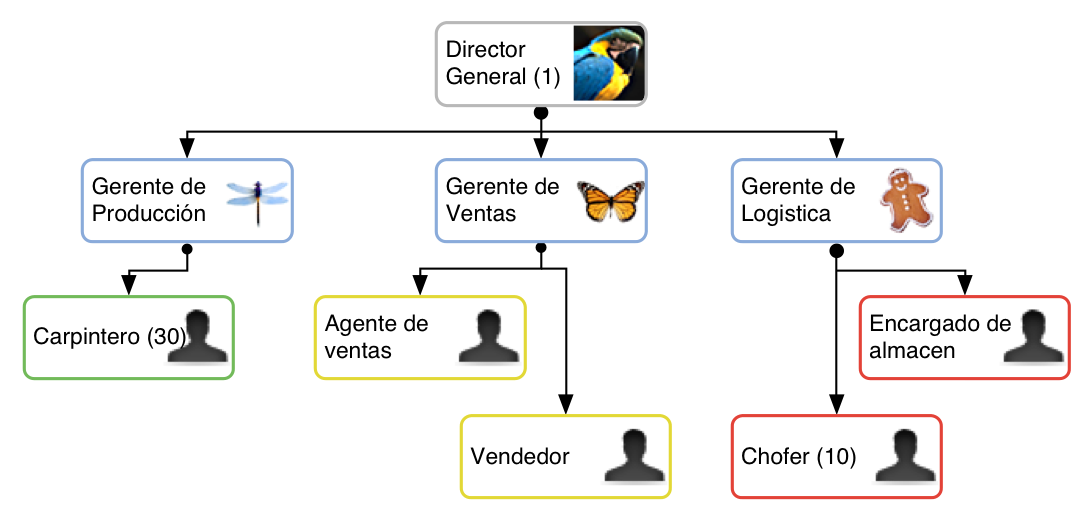
\includegraphics[width=.8\textwidth]{images/organigramaEm}
		\caption{Organigrama de la Mueblería Qetzal S. A. de C. V.}
		\label{fig:organigrama}
	\end{center}
\end{figure}


%---------------------------------------------------------
\section{Procesos involucrados}

\cdtInstrucciones{
	Coloque el mapa de procesos de la organización y liste a continuación los proceso que serán afectados por el desarrollo del sistema. Para cada proceso indique: Clave, Nombre y descripción.
}

\begin{figure}[htbp!]
	\begin{center}
		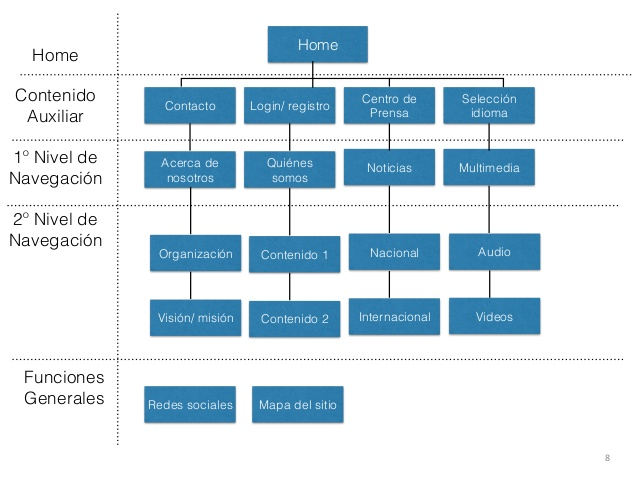
\includegraphics[width=.8\textwidth]{images/mapa}
		\caption{Mapa de procesos de la Mueblería Qetzal S. A. de C. V.}
		\label{fig:mapaProcASIS}
	\end{center}
\end{figure}

\begin{description}
	\item[PR-01] Nombre del proceso. Descripción del proceso.
\end{description}

%---------------------------------------------------------
\section{Requerimientos de usuario}

\cdtInstrucciones{
	Identifique y describa los requerimientos del usuario señalando: id, nombre, descripción y prioridad.
}

Los requerimientos del usuario son los siguientes\FootnoteStatus:

%\begin{requerimientosU}
%	\FRitem{RU-01}{Nombre del requerimiento}{Descripción del requerimiento.}{1}{\TODO}
%	\FRitem{...}{...}{...}{...}{...}
%\end{requerimientosU}

%---------------------------------------------------------
\section{Especificación de plataforma}	

\cdtInstrucciones{
	Coloque un diagrama y su descripción para aclarar el tipo de solución propuesta. \\
	
 En esta sección se debe aclarar:
	
\begin{description}
	\item[Tipo de sistema:] Web, aplicación móvil, de escritorio, híbrida, etc.
	\item[Software requerido:] Programas que se deberán instalar, desde el sistema operativo, compiladores, interpretes, servidores, etc.
	\item[Hardware requerido:] CPU, núcleos, velocidad, memoria, disco duro, etc.
	\item[servicios:] De conexión, seguridad, firewall, respaldo de energía, redundancia, uso de raids, etc.
\end{description}
}

\begin{figure}[htbp!]
	\begin{center}
		\fbox{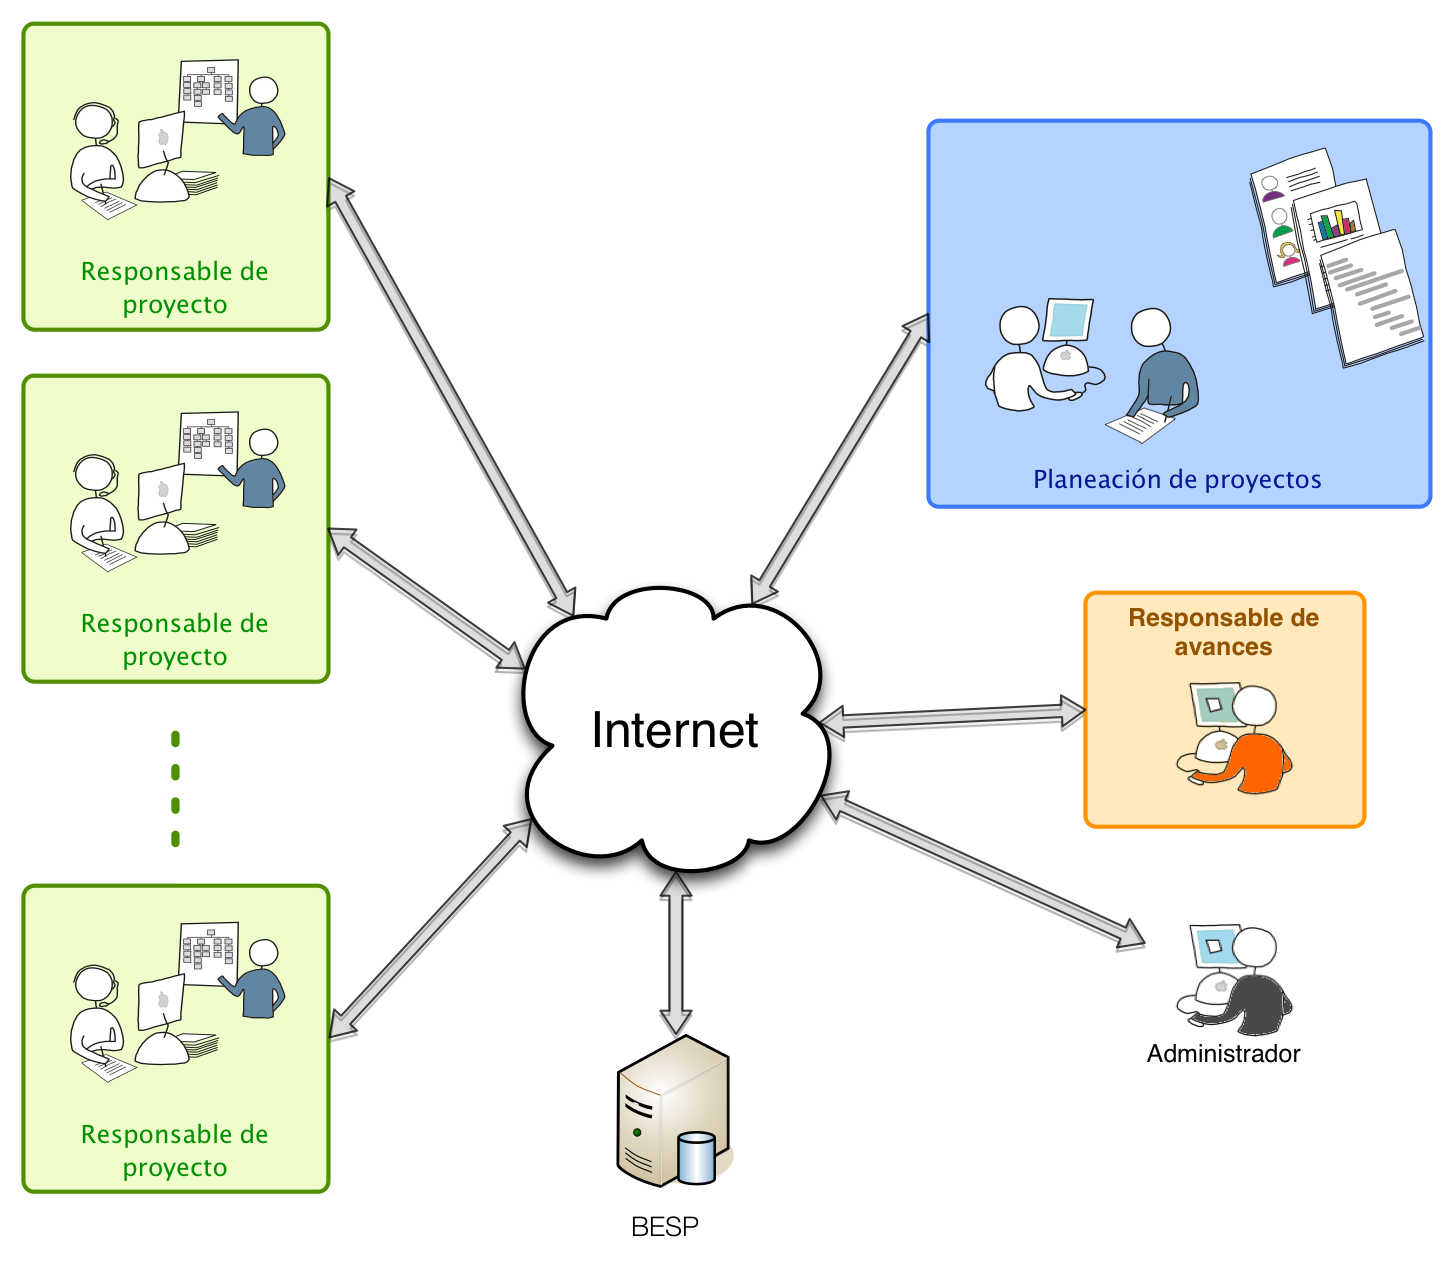
\includegraphics[width=.6\textwidth]{images/arquitectura}}
		\caption{Arquitectura del sistema.}
		\label{fig:arquitectura}
	\end{center}
\end{figure}

En la figura~\ref{fig:arquitectura} se describe la estructura del sistema, en ella se detalla ...


